\documentclass{article}

% Language setting
% Replace `english' with e.g. `spanish' to change the document language
\usepackage[english]{babel}

% Set page size and margins
% Replace `letterpaper' with `a4paper' for UK/EU standard size
\usepackage[letterpaper,top=2cm,bottom=2cm,left=3cm,right=3cm,marginparwidth=1.75cm]{geometry}

% Useful packages
\usepackage{amsmath}
\usepackage{graphicx}
\usepackage{subcaption} % For subfigures
\usepackage[colorlinks=true, allcolors=blue]{hyperref}
\usepackage{float}

\title{Machine Learning Exercise 1}
\author{Amélie Assmayr (12007770) \and
        Konstantinos Damanakis (12106343) \and
        Teresa Schuch (12007762)}

\begin{document}
\maketitle

\section{Introduction}
This report outlines the experimental design of the application of different classification algorithms across four diverse datasets. The goals is to show the trends in classifier performance, based on dataset properties like size and dimensionality, as well as the impact of preprocessing steps like scaling and different parameter settings.

The report is structured as followed: In Section 2 we introduce the chosen classifier and shortly explain their functionality. Section 3 describes the performance metrics used to evaluate each model across different configurations. Section 4 details the main characteristics of each datasets, the preprocessing steps applied and presents the evaluation results. Finally, in Section 5 discusses the main findings and insights drawn from the analysis.

\section{Classifiers}
We selected three distinct classifiers: an ensemble method (Random Forest), a margin-based method (SVM), and a distance-based method (KNN).

\subsection{K-nearest-neighbors}
\subsection{Random Forest}
Random Forest (RF) is an ensemble  method based on decision trees. It builds multiple decision trees during training and combines their prediction for more accurate and stable results. We chose this algorithm because it is good at handling both numerical and categorical data, making it a robust choice for diverse datasets. Furthermore due to its functionality Random Forests are resistant to overfitting, requires minimal preprocessing and offers offers flexibility through parameter tuning. This makes it useful also for complex and large datasets.


\subsection{Support Vector Machines} \label{svm}
Support Vector Machines (SVM) are supervised margin models that are based on finding the maximum-margin hyperplane that separates the classes. The optimal choice of hyperplane is the one that maximizes the distance (margin) from the support vectors (edge data points of each class). The higher the margin, the lower the generalization error of the classifier that is essential to avoid overfitting. The generalization error describes the the ability of the model to predict outcomes of new instances. The advantages of the SVM is its efficiency in high dimensional spaces and its versatility due to the use of kernels. On the other hand, the SVM is slow for large datasets and prone to overfitting if the number of features is much greater than the number of instances. In that case, a tuning of the parameters is critical.
\\
The Support Vector Machines use kernels, essentially mathematical functions that transform the data into a higher dimension. Typical kernel functions are "linear", "poly" (polynomial), "rbf" (radial basis function) or "sigmoid". Also, an important parameter is the regularization parameter (C) that is used to balance the maximization of the margin and the missclassification. High C decreases the margin and the missclassification while small C maximizes both. For the case of non-linear kernels (e.g rbf or poly), the parameter $\gamma$ is significant for the definition of decision boundary. Essentially, choosing a low gamma increases the influence of a training example on the nearby region of the feature space. On the other hand, a high gamma minimizes this influence, makes the decision boundary to be tight around individual points and as a result, favors the over-fitting.
\\
For the tests on the four datasets that are presented below, three different kernels have been tested, namely the linear, rbf and polynomial. The regularization parameter was set from the list [0.1, 1, 100, 1000], the hyperparameter $\gamma$ (only for non-linear kernels) was tuned according to the list [0.01, 1, 1000] and for the polynomial kernel degrees of 2,3 and 5 have been tested. In the following sections, a few exemplary results from these tests are shown.
\begin{table}[h!]
\centering
\begin{tabular}{||c c c c c c c c||} 
 \hline
 Kernel & C & $\gamma$ &d & Accuracy & Precision & Recall & F1 score \\ [0.5ex] 
 \hline\hline
 linear & 0.1 & - & - & 0.954 & 0.954 & 0.954 & 0.954 \\  
 rbf & 0.1 & 0.01 & - & 0.523 & 0.273 & 0.523 & 0.359 \\
 rbf & 1.0 & 0.01 & - & 0.977 & 0.978 & 0.977 & 0.977 \\
 rbf & 100 & 0.01 & - & 0.954 & 0.954 & 0.954 & 0.954 \\
 poly & 1.0 &  0.1 & 3 & 0.523 & 0.273 & 0.523 & 0.359 \\
 poly & 100 &  0.1 & 3 & 0.977 & 0.978 & 0.977 & 0.977 \\
  poly &  1.0&  1.0 & 5& 0.954 & 0.954 & 0.954 & 0.954 \\ [1ex] 
 \hline
\end{tabular}
\caption{Table including different used SVM parameters and the corresponding metrics.}
\label{table:votings_SVM}
\end{table}
\section{Performance Measures}
In order to ensure that the performance of the classifiers can be meaningfully compared, the following steps were taken:
\begin{itemize}
    \item \textbf{Dataset:} The same train/test splits were used across all classifiers to ensure consistency across all experiments.
    \item \textbf{Parameter changes:} To compare how one hyperparameter affects the outcome, only a single hyperparameter was changed at a time.
    \item \textbf{Baseline comparison:} The classifiers can be compared based on their baseline performance where no hyperparameters are set.
\end{itemize}

\subsection{Training time}
\subsection{Accuracy}
$\text{Formula} = \frac{TP + TN}{TP + TN + FP + FN}$

Accuracy measures the proportion of correctly classified instances out of all instances. While it’s easy to interpret, it can be misleading, especially in imbalanced datasets, because it doesn't distinguish between false positives and false negatives.

\subsection{Precision}
$\text{Formula} = \frac{TP}{TP + FP}$

Precision measures how many of the positive predictions were actually correct and therefore measures the model’s ability to precisely identify relevant instances within the data. Either by class or averaged across all classes.

\subsection{Recall}
$\text{Formula} = \frac{TP}{TP + FN}$

Recall measures how many true positive cases the model was able to identify. Either by class or averaged
across all classes.

\subsection{F1-score}

$\text{Formula}  = 2 \times \frac{\text{Precision} \times \text{Recall}}{\text{Precision} + \text{Recall}}$

The F1-score balances precision and recall. It thereby gives accurate results even if the dataset is skewed towards certain target classes. It might however be more difficult to immediately understand the score.

\section{Datasets}
PLOTS: Correlation and Barplot of Target

\subsection{Congressional Voting}
This dataset contains the voting records of U.S. House of Representatives members. It has 18 columns and 218 observation, making it one of the smaller datasets used. It includes voting data on 16 key issues, where each vote is recorded as "Yes," "No," or "Unknown." The target variable indicates whether each representative is a Democrat or Republican. Additionally, there is an ID column for each representative.


\subsubsection{Preprocessing}
First, a LabelEncoder is applied to convert the categorical variables into a binary format.  For the target variable, Democrats are encoded as 0 and Republicans as 1.  n the vote columns, 'no' is encoded as 0 and 'yes' as 1. Any 'unknown' values are replaced with NaN to mark them as missing. Next, rows with more than half of their values missing are removed from the dataset. The remaining missing values are then imputed by filling them with the most frequent value in each column. Since the dataset consists only of binary data, there is no need for additional transformations like scaling or outlier handling. 

\subsubsection{Results}

\subsubsection*{Support Vector Machines}
The classification of the preprocessed dataset with Support Vector Machines gives very high metrics over a different range of hyperparameters, as it can be seen in Table \ref{table:votings_SVM}. Either linear, rbf or polynomial kernels achieve high performance, if they are tuned to the right parameters. Also, the train times are very small for all of the kernels and parameter combinations. Both effectiveness and efficiency are satisfied, indicating that the preprocessed dataset has a clear structure.
\begin{table}[h!]
\centering
\begin{tabular}{||c c c c c c c c c||} 
 \hline
 Kernel & C & $\gamma$ &d & Accuracy & Precision & Recall & F1 score & Train time [ms] \\ [0.5ex] 
 \hline\hline
 linear & 0.1 & - & - & 0.954 & 0.954 & 0.954 & 0.954 & 9 \\  
 rbf & 0.1 & 0.01 & - & 0.523 & 0.273 & 0.523 & 0.359 & 14 \\
 rbf & 1.0 & 0.01 & - & 0.977 & 0.978 & 0.977 & 0.977 & 12\\
 poly & 1.0 &  0.1 & 3 & 0.523 & 0.273 & 0.523 & 0.359 & 12 \\
 poly & 100 &  0.1 & 3 & 0.977 & 0.978 & 0.977 & 0.977 & 8 \\
 poly &  1.0&  1.0 & 5& 0.954 & 0.954 & 0.954 & 0.954 & 9 \\ [1ex] 
 \hline
\end{tabular}
\caption{Table including different used SVM parameters and the corresponding metrics.}
\label{table:votings_SVM}
\end{table}
\\
Among the parameters that were tested, the model has lower performance for non-linear kernels when the gamma hyperparameter is set too low. In particular, the model has a poorer performance for the rbf kernel, when the combination of $\gamma$ = 0.01 and C = 0.1 is used, and for poly kernel, when $\gamma$ = 0.1 and C $<$ 1.0. Using small $\gamma$, smoothens the decision boundary and oversimplifies the model that consequently for this given dataset, fails to classify correctly the different patterns. This is observed also for the rbf kernel, however when choosing C $\ge$ 1, due to the fact that the missclassifications are minimized, the performance of the model is improved in classifying the data. 
\\Performing the hyperparameter tuning with the scikit function GridSearchCV with the same input ranges as in the manual investigation, a linear kernel with C = 0.1 gives the highest accuracy of 0.970. The holdout method estimates slightly lower value as shown in Table \ref{table:votings_SVM_cross} but this should be related to the different splitting as well as the averaging that is performed by the GridSearchCV method.
\\ Table \ref{table:votings_SVM_cross} shows a comparison of the metrics between the hold-out and the 10-fold cross-validation method, for linear kernel and C = 1. A small improvement of effectiveness is observed with the cross-validation method that can be due to the fact that this method averages the performance over different splits. 
\begin{table}[h!]
\centering
\begin{tabular}{||c c c c c||} 
 \hline
Method &  Accuracy & Precision & Recall & F1 score \\ [0.5ex] 
 \hline\hline
hold-out & 0.954 & 0.954 & 0.954 & 0.954  \\  
 10-fold cross validation &  0.959&  0.963 &  0.959& 0.9659 \\ [1ex] 
 \hline
\end{tabular}
\caption{Table including comparison of metrics for hold-out and 10-fold cross validation method, for linear kernel and C = 1.}
\label{table:votings_SVM_cross}
\end{table}
\subsection{Amazon Reviews}
The amazon reviews dataset includes 10002 columns and 740 rows. The large number of columns makes its classification quite challenging. Besides the, column 'ID' that includes the ascending number of row, there are 10000 columns that include an integer number between 0 and 32. The target variable ("Class") contains categorical data that are associated to names of famous authors such as "Bukowski", "Shea" etc. Although, the names of the columns do not clearly indicate what the integer values describe, it could be assumed that they represent the result of a counting.
\begin{figure}[htp]

\centering
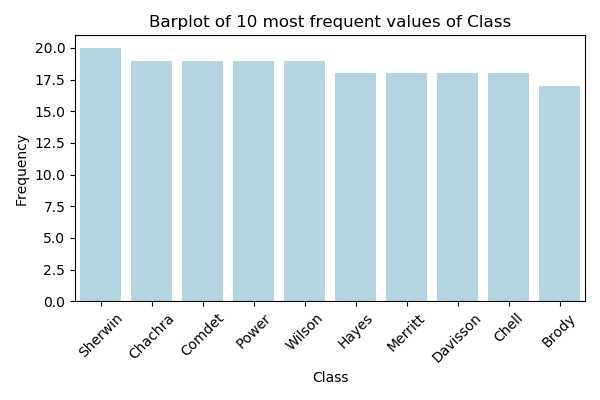
\includegraphics[width=.5\textwidth]{reviews_class.png}
\caption{Barplot including 10 most frequent classes of output variable.}
\label{fig:barplot_reviews}
\end{figure}
\begin{figure}[htp]

\centering
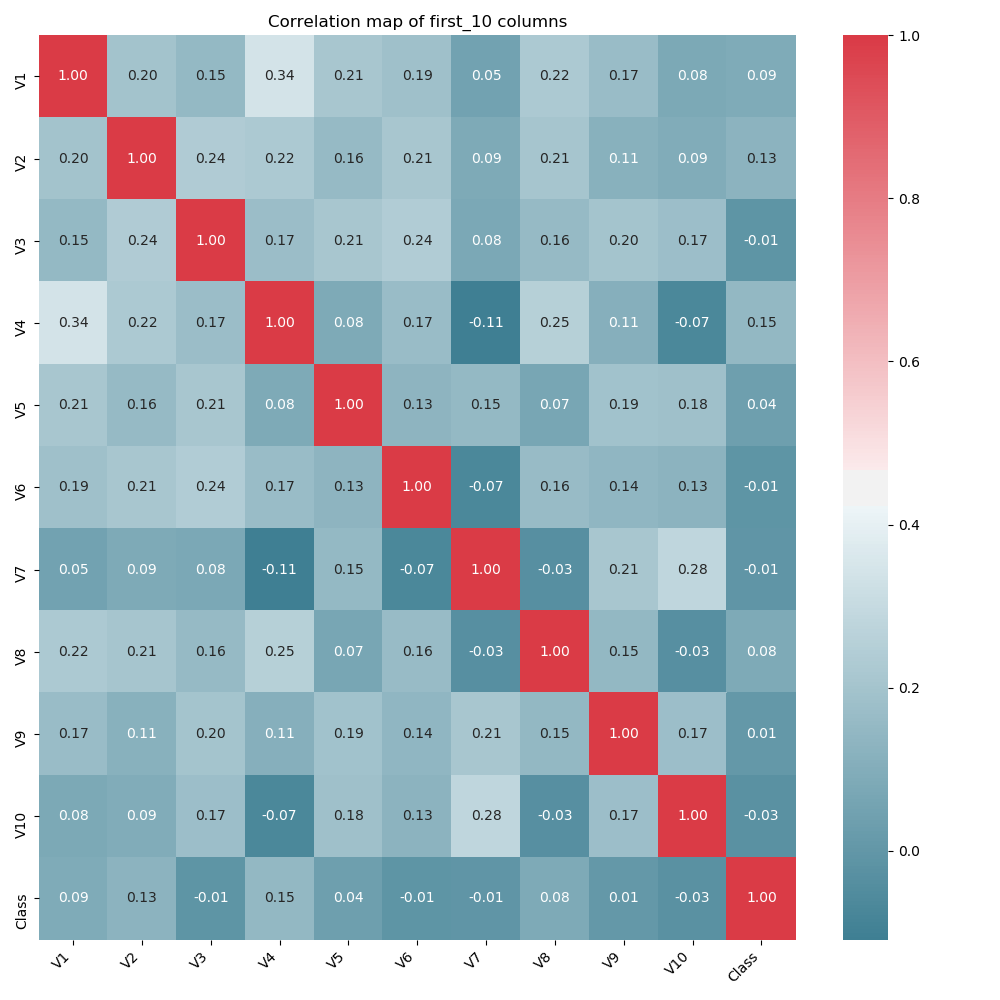
\includegraphics[width=.3\textwidth]{correlation_map_first_10.png}\hfill
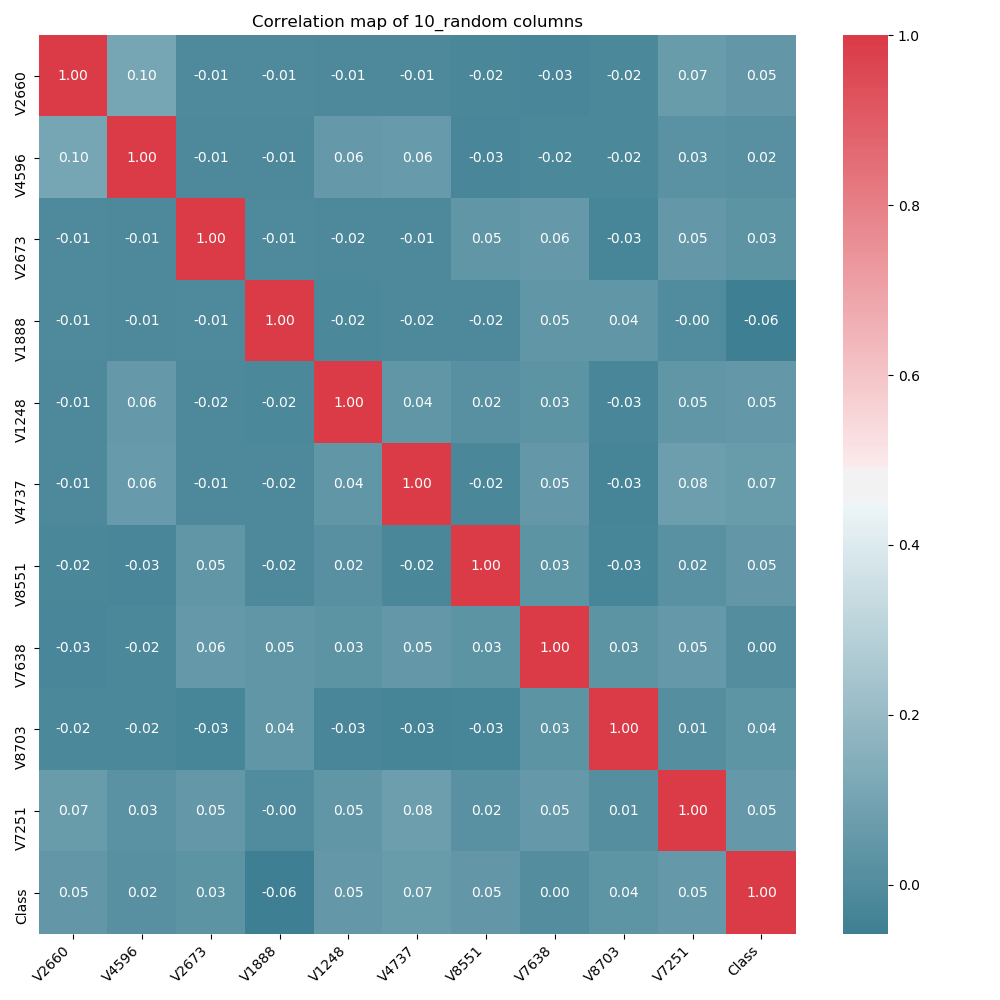
\includegraphics[width=.3\textwidth]{correlation_map_10_random.png}\hfill
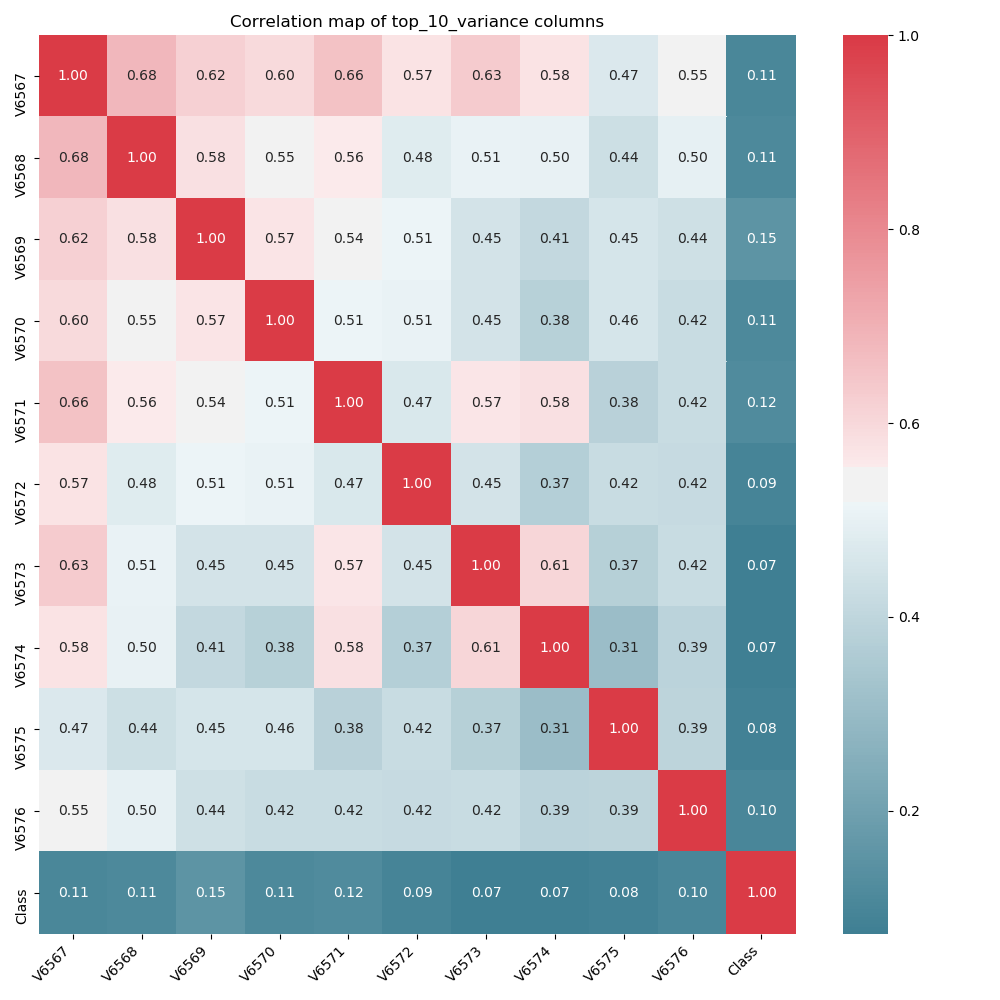
\includegraphics[width=.3\textwidth]{correlation_map_top_10_variance.png}

\caption{Correlation plot including the class and first 10 columns (left), 10 random columns(middle), 10 columns with largest variance (right).}
\label{fig:correlation_reviews}

\end{figure}
\subsubsection{Preprocessing}
Since all columns have integer types, except from the "Class", no encoding is necessary for the preprocessing of this dataset. The data neither feature any missing values nor any obvious outliers. Despite scaling of the data is not a necessary step, a standarization scaling is used.
\subsubsection{Results}

\subsubsection*{Support Vector Machines}

The metrics for the dataset as classified by Support Vector Machines over different model parameters (kernel function, C, gamma, degree of polynomial) are presented in table \ref{table:reviews_SVM}. The processing time is quite large for this dataset which is expected due to the large number of features and therefore, the complexity of the calculations. It is clear that effectiveness is relatively low for that classifier and dataset. Among the three different kernels, the linear shows the best performance in terms of performance. It is interesting that for a given kernel, tuning parameters such as C and $\gamma$ and using different ranges, seems to have no impact on the metrics. For the polynomial kernels, a second degree shows the highest metrics, however they are still very low. It should be noted that a standarization of the dataset has been performed before splitting the dataset. It is possible that the dataset includes a significant number of irrelevant features that apart from increasing the computing time, they impact and more precisely, saturate the accuracy when different hyperparameters are chosen. In that case, feature selection becomes an important step in order to optimize the performance of the model. 
\begin{table}[h!]
\centering
\begin{tabular}{||c c c c c c c c c||} 
 \hline
 Kernel & C & $\gamma$ &d & Accuracy & Precision & Recall & F1 score & Train time [ms]\\ [0.5ex] 
 \hline\hline
 linear & 1.0 & - & - & 0.606 & 0.704 & 0.606 & 0.611 &56049\\ 
 rbf & 100 & 0.01 & - & 0.013 & 0.0002 & 0.013 & 0.004 & 61713\\
 poly & 0.1 &  1.0 & 3 & 0.060 & 0.042 & 0.060 & 0.024 & 56398\\
 poly & 1.0 &  1.0&  2 & 0.073 & 0.055 & 0.733 & 0.039& 53921 \\ [1ex] 
 \hline
\end{tabular}
\caption{Table including different used SVM parameters and the corresponding metrics.}
\label{table:reviews_SVM}
\end{table}
\\
The table \ref{table:reviews_SVM_cross} compares the acquired metrics between hold-out and 10-fold cross-validation method. 
\begin{table}[h!]
\centering
\begin{tabular}{||c c c c c||} 
 \hline
Method &  Accuracy & Precision & Recall & F1 score \\ [0.5ex] 
 \hline\hline
hold-out & 0.606 & 0.704 & 0.606 & 0.611  \\  
 10-fold cross validation &  0.567&  0.517 & 0.567& 0.509 \\ [1ex] 
 \hline
\end{tabular}
\caption{Table including comparison of metrics for hold-out and 10-fold cross validation method, for linear kernel and C = 1.}
\label{table:reviews_SVM_cross}
\end{table}
\\
Using the GridSearchCV method, the parameters that maximize the performance of the model is a linear kernel and C = 0.1, for which the accuracy obtained by cross-validation is 0.52. For the same parameters, the hold-out method gives an accuracy of 0.606.
\\
Further investigation was performed on the dataset in order to improve the metrics. In particular, two techniques were applied: oversampling and dimension reduction. After oversampling the data, the cross-validation gives an accuracy of 0.72 and a precision 0.742 for linear kernel and C = 1.0. With data scaling, the former goes up to 0.808 and the latter up to 0.847. With the dimension reduction method, an accuracy of 0.487 and a precision 0.473 is achieved. 

\subsection{Road Traffic Accidents}
\subsubsection{Preprocessing}
\subsubsection{Results}

\subsubsection*{Support Vector Machines}
The metrics in Table \ref{table:rta_SVM} show that for either linear, rbf or poly kernels a high precision and accuracy is achieved with the proper parameter combinations. It is interesting that the best performance parameters show a saturation in such a way that applying different kernels does not change the metrics. The train time is significant for all of the kernels shown in \ref{table:rta_SVM} when the hold-out method is used. For the linear kernels, the processing time scales up when selecting C$>$1, rendering the computational cost not optimal. For rbf and poly kernels, a wider range of the hyperparameter C can be tested within a meaningful processing time, only when gamma is set low, such as $\gamma$ = 0.01 or vice-verca, a wider range of gamma can be tested only when C is chosen to be small (e.g C $\le$1). Larger values of $\gamma$ and C can increase the computational time, with the former forcing the model to define a decision boundary more tight around individual points, as mentioned in section \ref{svm}, and the latter leads to stricter fitting of the data. 
\\ 
 
\begin{table}[h!]
\centering
\begin{tabular}{||c c c c c c c c c||} 
 \hline
 Kernel & C & $\gamma$ &d & Accuracy & Precision & Recall & F1 score & Train time [ms] \\ [0.5ex] 
 \hline\hline
 linear &  1.0 & - & - & 0.857 & 0.734 & 0.857 & 0.790 & 5095 \\
  rbf &  1.0 & 0.01 & - & 0.857 & 0.734 & 0.857 & 0.790 & 18852\\
 poly &  0.1 & 0.01 & 3 & 0.857 & 0.734 & 0.857 & 0.790 & 5751 \\[1ex] 
 \hline
\end{tabular}
\caption{Table including different used SVM parameters and the corresponding metrics.}
\label{table:rta_SVM}
\end{table}
\\
Table \ref{table:rta_SVM_cross} shows the comparison of the metrics between the hold-out and the 10-fold cross-validation method, for linear kernel and C = 1.
\begin{table}[h!]
\centering
\begin{tabular}{||c c c c c||} 
 \hline
Method &  Accuracy & Precision & Recall & F1 score \\ [0.5ex] 
 \hline\hline
hold-out & 0.856 & 0.734 & 0.856 & 0.790  \\  
 10-fold cross validation &  0.842&  0.710 & 0.842& 0.770 \\ [1ex] 
 \hline
\end{tabular}
\caption{Table including comparison of metrics for hold-out and 10-fold cross validation method, for linear kernel and C = 1.}
\label{table:rta_SVM_cross}
\end{table}
\\ 
When searching for the optimal parameters with GridSearchCV, an accuracy of 0.844 can be achieved with rbf kernel, C = 1 and $\gamma$ = 0.1. The hold-out method with the same parameters gives an accuracy of 0.857. 
\\ It should be noted that the method of oversampling was used to investigate its impact on the metrics. For linear kernel and C = 1.0, the accuracy is 0.485, value that is significantly lower than the metrics without oversampling.   
\subsection{Machine Failure}
\subsubsection{Preprocessing}
\subsubsection{Results}
\subsubsection*{Support Vector Machines}
Table \ref{table:machine_SVM} shows some exemplary results for different combinations of input hyperparameters. All three kernels give high accuracy and precision if the parameters are tuned carefully. A selection of linear kernel gives high metrics for different ranges of C. For rbf kernel, choosing $\gamma$=0.01 for different C parameters gives a good precision and accuracy but this is not the case for larger $\gamma$. Processing time is small for most of the combinations, however as gamma grows beyond 0.01, the accuracy and precision deteriorate and classification seems to be more prone to overfitting. Regarding the polynomial kernel and degree$=$3, the accuracy is high for most of the tested parameters, except from low $\gamma$ and C. Effectiveness decreases with $\gamma$ which is an indication of underfitting. In general, this different behavior when varying the kernel implies some complexity within the dataset. Nevertheless, for every kernel, the hyperparameters can be tuned accordingly in order to achieve high metrics. Linear kernel performs better in terms of efficiency and training time.

\begin{table}[h!]
\centering
\begin{tabular}{||c c c c c c c c c||} 
 \hline
 Kernel & C & $\gamma$ &d & Accuracy & Precision & Recall & F1 score & Train time [ms] \\ [0.5ex] 
 \hline\hline
 linear & 0.1 & - & - & 0.878 & 0.878 & 0.878 & 0.878 & 31 \\
 linear & 100 & - & - & 0.883 & 0.883 & 0.883 & 0.883 & 1066 \\
 rbf & 0.1 & 0.01 &- &  0.888 & 0.888 & 0.888 & 0.888 & 120  \\
 rbf & 0.1 & 1.0 & - & 0.539 & 0.291 & 0.539 & 0.378 & 197 \\
 poly & 0.1 &  1.0 &  3 & 0.878 & 0.880 &  0.878 & 0.878 & 142  \\ 
 poly & 1.0 &  0.01 &  3 & 0.540 & 0.291 &  0.540 & 0.378 & 75  \\[1ex] 
 \hline
\end{tabular}
\caption{Table including different used SVM parameters and the corresponding metrics.}
\label{table:machine_SVM}
\end{table}
\\ 
Table \ref{table:machine_SVM_cross} shows the comparison of the metrics between the hold-out and the 10-fold cross-validation method, for linear kernel and C=1. The metrics estimated after the 10-fold cross-validation method is used are slightly higher, in the order of 5$\%$, in comparison to the hold-out method. 
\begin{table}[h!]
\centering
\begin{tabular}{||c c c c c||} 
 \hline
Method &  Accuracy & Precision & Recall & F1 score \\ [0.5ex] 
 \hline\hline
hold-out & 0.883 & 0.883 & 0.883 & 0.883  \\  
 10-fold cross validation &  0.915&  0.916 & 0.915& 0.915 \\ [1ex] 
 \hline
\end{tabular}
\caption{Table including comparison of metrics for hold-out nad 10-fold cross validation method, for linear kernel and C = 1.}
\label{table:machine_SVM_cross}
\end{table}
\\
In addition, the estimation of the best parameter with GridSearchCV function gives an accuracy of 0.921 with rbf kernel, C = 1 and gamma = 0.01. This estimate is slightly higher than the one of hold-out method for the same parameters, which gives an accuracy of 0.873. This is explained because of the difference between the way the splitting and averagin is performed by these two methods, as mentioned above.
\section{Discussion of Findings}



\section{Notes}

\end{document}